% !TEX root = 00_main_aaai_2027.tex
% CS197 six-move introduction; provenance: papers/analysis/canonical_validity.json, papers/analysis/decomp_cis.json, papers/analysis/free_baseline.json.
\section{Introduction}
\label{sec:intro}

% Move 1: problem motivation.
Automated benchmarks for autonomous scientific discovery and reasoning routinely ship a worked gold reference alongside each task~\citep{hendrycks2021math,cobbe2021gsm8k,chen2021codex}.
Paying a frontier large language model (LLM) judge to grade every candidate trace is costly, and judge prompts often inject unmeasured variance~\citep{zheng2023judging,tan2024judgebench}.
Benchmark builders therefore look for deterministic, judge-free evaluators derived directly from the gold reference.
However, a student or research agent who writes a plausible wrong derivation can match the gold reference closely, whereas a valid solution using an alternative strategy can diverge in surface form.

% Move 2: prior assumption.
Prior work frames automated evaluation along a single cost-versus-quality spectrum, placing lexical and embedding metrics at the cheap end~\citep{yuan2021bartscore} and LLM judges at the expensive end~\citep{liu2023geval,zheng2023judging}.
This framing implicitly assumes that reference similarity degrades gracefully as cost falls.
The sharpest judge-free candidate is teacher-forced accuracy (\tfa), proposed by \textsc{Putnam-AXIOM}~\citep{gulati2025putnam}: feed the model the problem and gold reference token by token, and measure the fraction of gold tokens predicted greedily by argmax.
While \textsc{Putnam-AXIOM} validated \tfa{} as a model-level ranker, it left untested whether \tfa{} or related similarity metrics grade individual solutions~\citep{gulati2025putnam}.

% Move 3: conceptual contribution.
We challenge that cost-versus-quality spectrum and argue that the operative distinction in reference-based evaluation is \emph{mechanism} rather than cost.
Metrics that score resemblance to reference text (\emph{reference-matching metrics}) behave fundamentally differently from signals that test whether a candidate satisfies an executable or symbolic endpoint (\emph{verification signals}).
Because a reference-matching score is dominated by how predictable the reference text is---a quantity fixed before any candidate is generated---it grades the answer key rather than the student.

% Move 4: concrete instantiation + Figure 1.
We establish this mechanism across seventeen instruction-tuned models from four model families on eight math and code benchmarks plus an agentic software patch setting, anchored to sixty blind human-graded \textsc{MATH-500} solutions on separate \emph{reasoning soundness} and \emph{writing style} scales and $492$ executed \textsc{HumanEval}/\textsc{MBPP+} solutions (Figure~\ref{fig:class}).
We separate signals along three diagnostics: per-task validity against blind human soundness and executed unit tests, a cross-family fixed-effects variance decomposition backed by causal reference interventions, and a cross-benchmark ranking boundary map from olympiad problems to saturated grade-school tasks.

\begin{figure}[t]
\centering
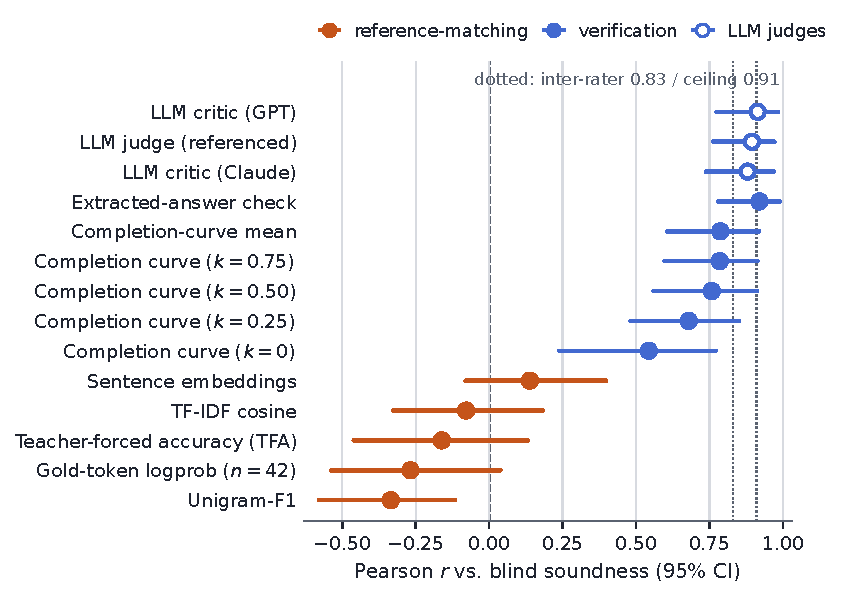
\includegraphics[width=\columnwidth]{figures/fig_class.pdf}
\caption{\textbf{Every untrained reference-matching metric straddles zero or trends negative against blind human soundness, whereas verification signals track soundness and an extracted-answer check leads the field at $+0.92$.} Pearson $r$ with $2{,}000$-resample $95\%$ bootstrap confidence intervals (CIs) on the sixty-task \textsc{MATH-500} anchor set (gold-token logprob on $n{=}42$ tasks with logprobs available; LLM judges shown as expensive reference points).
Dotted lines mark the same-rubric external inter-rater agreement ($r = 0.83$, $n{=}30$) and implied single-rater ceiling ($0.91$, indicative only due to wide CIs).}
\label{fig:class}
\end{figure}

% Move 5: headline evaluation summary.
Every untrained reference-matching metric we tested fails to grade individual solutions, sitting inside $[-0.33, +0.14]$ against human soundness and $[0.00, +0.17]$ against executed code tests, because $83$--$92\%$ of per-solution \tfa{} variance is a shared cross-family item effect driven by \emph{reference perplexity} ($r = -0.895$).
Averaging across tasks cancels that shared item effect, allowing aggregate ranking on hard olympiad sets ($\rho = +0.86$ on \textsc{Omni-MATH}), yet the ranking collapses under a pre-registered length-matched boilerplate control ($\Delta\rho = +0.41 \; [+0.35, +0.46]$) and inverts on saturated benchmarks.
Meanwhile, the zero-cost machine-checked \emph{extracted-answer check} reaches $r = +0.92 \; [+0.78, +0.99]$ against soundness and outperforms a thirty-two-rollout Monte-Carlo \emph{completion curve} ($r = +0.79$, paired $\Delta r = +0.13 \; [+0.05, +0.24]$).

% Move 6: implications + contributions.
These findings explain why benchmark builders should reserve gold references for endpoint verification rather than untrained similarity scoring, and provide a lightweight reference-perplexity check before trusting leaderboard rankings; full boundary tables, post-hoc baselines, and rubric specifications appear in Appendices~\ref{app:boundary}--\ref{app:rubric}.
We make the following contributions:
\begin{enumerate}
\item We establish a per-task grading null across five primary and three post-hoc untrained reference-matching metrics against blind human soundness ($[-0.33, +0.14]$) and executed unit tests ($[0.00, +0.17]$).
\item We identify the mechanism via cross-family fixed-effects decomposition ($83$--$92\%$ item share, $r = -0.895$ with reference perplexity) and confirm it through an answer-line intervention, a pre-registered length-matched boilerplate control, and two failed repair sweeps.
\item We map the aggregate ranking boundary across nine datasets and twenty-four within-family ladders, and show that no cheap verification signal tested beats the zero-cost extracted-answer check on tasks with extractable answers.
\end{enumerate}
